\subsection{Deep Learning using Functional Geometric Monitoring (FGM) protocol}\label{subsec:deep-learning-using-fgm-protocol}

\begin{frame}{Definitions}
    \begin{block}{Definition (Safe function for admissible region $A$)}
        A function $\phi :\mathbb{R}^d\rightarrow \mathbb{R}$ such that, for every $n$, and every $\pmb{X}_i$, i \in [\,1,n]\,\\
        \vspace{0.1cm}
        \begin{center}
            $\sum_{i=1}^n\phi (\pmb{W}_i) \leq 0$\hspace{0.4cm}$\Longrightarrow$\hspace{0.4cm}$\frac{1}{n}\sum_{i=1}^n\pmb{W}_i\in A$
        \end{center}
    \end{block}
    \vspace{0.4cm}
    \begin{columns}
        \column{0.65\textwidth}
        \begin{itemize}
            \item[]{The FGM protocol [Samoladas et al. 2018] monitors the condition $\sum_{i=1}^n\phi (\pmb{W}_i) \leq 0$.}
        \end{itemize}
        \column{0.35\textwidth}
        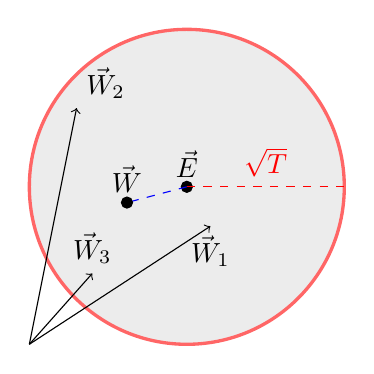
\begin{tikzpicture}
            \filldraw[color=red!60, fill=gray!50, fill opacity=0.3, very thick](0,0) circle (2);
            \coordinate (E) at (0,0);
            \coordinate (u1) at (0.3,-0.5);
            \coordinate (u2) at (-1.4,1.0);
            \coordinate (u3) at (-1.2,-1.1);
            \draw [fill] (E) circle (0.2em) node [anchor=south] {$\vec{E}$};
            \draw [->,thin] (-2,-2)--(u1)  node [anchor=north]{$\vec{W}_1$};
            \draw [->,thin] (-2,-2)--(u2) node [anchor=south west] {$\vec{W}_2$};
            \draw [->,thin] (-2,-2)--(u3) node [anchor=south]
            {$\vec{W}_3$};
            \coordinate (x) at (-0.76,-0.2);
            \draw [blue,dashed] (E)--(x);
            \draw [fill] (x) circle (0.2em) node [anchor=south] {$\vec{W}$};
            \draw [red,dashed] (E)--(2,0) node [pos=0.5, anchor=south] {$\sqrt{T}$};
        \end{tikzpicture}
    \end{columns}
\end{frame}

\begin{frame}{Correspondence with GM protocol}
    \setbeamertemplate{itemize items}[circle]
    \begin{itemize}
        \item{The \textbf{admissible region} in GM protocol (M. Kamp) is the \textbf{convex set}
        \newline
        \begin{center}
            $A=\{\pmb{W}_i\in\mathbb{R}^d\:\:|\:\:||\pmb{W}_i-\pmb{E}||_2^2 - T \leq 0\}$
        \end{center}
        }
        \vspace{0.4cm}
        \item{Samoladas et al. constructed the concave function $\phi:\mathbb{R}^d\rightarrow\mathbb{R}$ that is safe for $A$ as
        \newline
        \begin{center}
            $\phi(\pmb{W_i},\pmb{E}) = \max\{-T||\pmb{E}|| - \pmb{W_i}\frac{\pmb{E}}{\pmb{||E||}}, ||\pmb{W_i}+\pmb{E}|| - (1+T)||\pmb{E}||\}$
        \end{center}
        We can call this function as \textbf{’spherical cap’}.
        }
        \vspace{0.4cm}
        \item{Finally, the coordinator monitors the condition,
        \newline
        \begin{center}
            $\sum_{i=1}^n\phi(\pmb{W}_i,\pmb{E}) \leq 0$
        \end{center}
        }
    \end{itemize}
\end{frame}

\begin{frame}{The FGM Protocol (1)}
    \begin{columns}
        \column{0.5\textwidth}
        \setbeamertemplate{itemize items}[circle]
        \begin{itemize}
            \item{At the \textbf{beginning} of a round,
            \vspace{0.2cm}
            \setbeamertemplate{itemize items}[square]
            \begin{itemize}
                \item{The coordinator knows the model parameters from all workers $\pmb{W}_i$.}
                \vspace{0.3cm}
                \item{The coordinator ships the estimate $\pmb{E}$ to all workers.}
                \vspace{0.3cm}
                \item{Each site calculates $\phi$ from $\pmb{E}$.}
                \vspace{0.3cm}
                \item{Each site initializes $\pmb{W}_i=\pmb{E}$.}
            \end{itemize}
            }
        \end{itemize}
        \column{0.5\textwidth}
        \begin{figure}
            \includegraphics[width=8.5cm,height=6cm,center]{images/ml-fgm-2.png}\label{fig:ml-fgm-1}
        \end{figure}
    \end{columns}
\end{frame}

\begin{frame}{The FGM Protocol (2)}
    \begin{columns}
        \column{0.5\textwidth}
        \vspace{-1cm}
        \setbeamertemplate{itemize items}[circle]
        \begin{itemize}
            \item{\textbf{During} a round,
            \vspace{0.2cm}
            \setbeamertemplate{itemize items}[square]
            \begin{itemize}
                \item{Each worker updates $\pmb{W}_i$ by fitting a batch of samples.}
                \vspace{0.3cm}
                \item{The coordinator monitors the following condition,\\
                \begin{center}
                    $\psi = \sum_{i=1}^n\phi(\pmb{W}_i,\pmb{E}) \leq 0$
                \end{center}
                }
            \end{itemize}
            }
        \end{itemize}
        \column{0.5\textwidth}
        \begin{figure}
            \includegraphics[width=8.5cm,height=6cm,center]{images/ml-fgm-2.png}\label{fig:ml-fgm-2}
        \end{figure}
    \end{columns}
\end{frame}

\begin{frame}{The FGM Protocol (3)}
    \begin{columns}
        \column{0.5\textwidth}
        \vspace{-1cm}
        \setbeamertemplate{itemize items}[circle]
        \begin{itemize}
            \item{At the \textbf{end} of a round,
            \vspace{0.2cm}
            \setbeamertemplate{itemize items}[square]
            \begin{itemize}
                \item{The coordinator receives from each worker the current $\pmb{X}_i$.}
                \vspace{0.3cm}
                \item{The coordinator calculates the new estimate ($\pmb{E}$) and quantum ($\pmb{\theta}$).}
            \end{itemize}
            }
        \end{itemize}
        \column{0.5\textwidth}
        \begin{figure}
            \includegraphics[width=8.5cm,height=6cm,center]{images/ml-fgm-2.png}\label{fig:ml-fgm-3}
        \end{figure}
    \end{columns}
\end{frame}

\begin{frame}{Contribution}
    \setbeamertemplate{itemize items}[circle]
    \begin{itemize}
        \item{Michael Kamp et al. had not tested their method in this type of NNs.}
        \vspace{1cm}
        \item{We attempt to train these difficult networks distributedly by a more efficient method.}
    \end{itemize}
\end{frame}